\chapter{Architetture Parallele}

Per aumentare ancora di più le prestazioni, se è già stato applicato tutto ciò descritto in precedenza, si deve ricorrere a un'architettura dotata di più unità computazionali in modo da avere un \fancyglitter{parallelismo esplicito}. 

\nt{Preso in considerazione il fatto che i programmi debbano andare riscritti per girare su più core.}

\section{I Problemi del Parallelismo Esplicito}

Tuttavia, (eccetto che in casi molto molto particolari) l’incremento di
prestazioni (il cosiddetto \fancyglitter{speed-up}) che si può ottenere usando più
CPU su cui far girare in parallelo i vari programmi è meno che
lineare rispetto al numero di CPU disponibili. Principalmente perché i programmi che girano in parallelo dovranno sincronizzarsi tra loro. Consideriamo il comando "gcc main.c function1.c function2.c -o output". Supponiamo che, lanciando il programma su una macchina monoprocessore ci vogliano 7 secondi: 

\begin{itemize}
  \item 3 secondi per compilare main.c 
  \item 2 secondi per compilare function1.c 
  \item 1 secondo per compilare function2.c 
  \item 1 secondo per linkare gli oggetti. 
\end{itemize}

\paragraph{}
Con 3 CPU a disposizione i tre sorgenti possono essere compilati in parallelo, ma l'operazione di linking può essere eseguita solo dopo che tutti e tre gli oggetti sono stati generati (quindi dopo 3 secondi). In questo modo il tempo si riduce da 7 a 4 secondi con uno speed-up di 1.75 pur avendo usato 3 processori.
\begin{figure}[h]
    \centering
    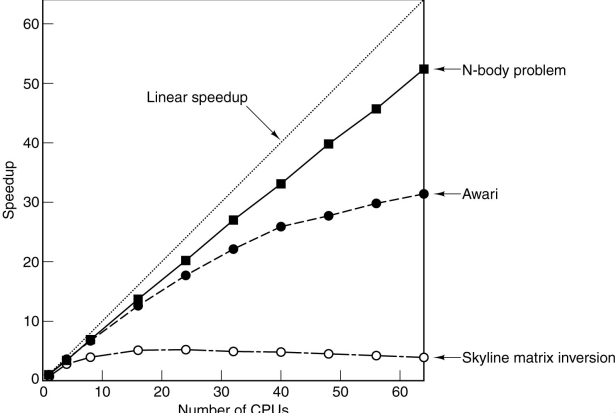
\includegraphics[width=0.3\textwidth]{04-ArchitettureParallele/speed-up.png}
    \caption{Speed-up di alcuni problemi computazionali.}
\end{figure}
\pagebreak
\begin{figure}[!h]
    \centering
    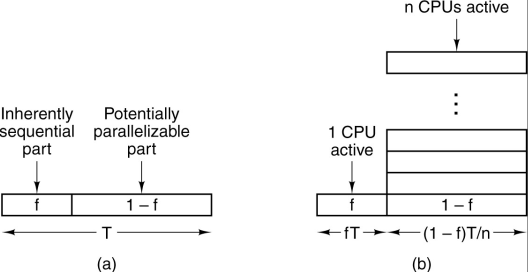
\includegraphics[scale=0.7]{04-ArchitettureParallele/Parallelizzazione limiti.png}
    \caption{Sia P un programma che gira in tempo T su una CPU, con f = la
frazione di T dovuta a codice sequenziale, e (1-f) la frazione di T
dovuta a codice parallelizzabile.}
\end{figure}

\nt{Il tempo di esecuzione dovuto alla parte parallelizzabile, passa
da (1-f)T a (1-f)T/n se sono disponibili n processori. Questa è nota come \fancyglitter{legge di Amdahl}}

\begin{figure}[h]
    \centering
    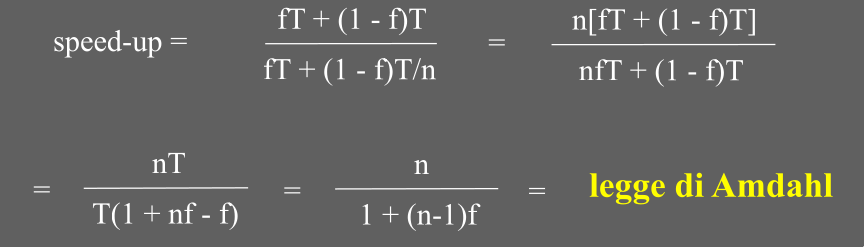
\includegraphics[scale=0.5]{04-ArchitettureParallele/Legge di Amdahl.png}
    \caption{La legge di Amdahl.}
\end{figure}

\begin{itemize}
  \item Se si vuole ottenere uno speed-up perfetto, pari al numero di CPU usate, f deve valere 0, ma ciò è impossibile. 
  \item Spesso il miglioramento è sub-lineare.
\end{itemize}

\paragraph{I problemi del parallismo esplicito sono generalmente due:}

\begin{enumerate}
  \item La quantità limitata di parallelismo nel codice dei programmi (problema software). 
  \item Gli elevati costi delle comunicazioni tra processori e memoria (problema hardware).
\end{enumerate}

\nt{Per molte applicazioni avere uno speed-up, seppur limitato, è comunque accettabile, perché: 
\begin{itemize}
  \item La presenza di più processori aumentà l'affidabilità del sistema. 
  \item Servizi che per loro natura sono forniti su ampia scala geografica,
devono essere implementati con una architettura distribuita. Se il
sistema fosse centralizzato in un unico nodo, l’accesso di tutte le
richieste a quest’unico nodo costituirebbe probabilmente un collo
di bottiglia in grado di rallentare enormemente il servizio fornito.
\end{itemize}
}

\paragraph{Ci sono tre tipi di architetture parallele esplicite:}

\begin{itemize}
  \item Multi-threading (a). 
  \item Sistemi a memoria condivisa (b, c). 
  \item Sistemi a memoria distribuita (d, e).
\end{itemize}

\begin{figure}[h]
    \centering
    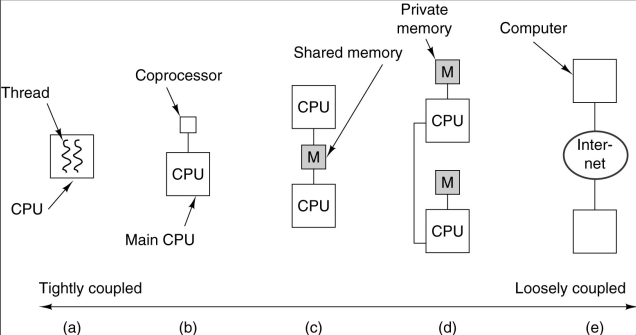
\includegraphics[scale=0.5]{04-ArchitettureParallele/PE.png}
    \caption{Vari tipi di architetture esplicitamente parallele.}
\end{figure}

\section{Multi-Threading}

\subsection{Introduzione}

\dfn{Architettura Multi-Threaded}{
  Una CPU multi-threaded è una architettura parallela un po’
particolare, in quanto il multi-threading è realizzato con un’unica
CPU (sempre single core), ma porta il programmatore
a concepire e sviluppare le sue applicazioni come formate da un
insieme di programmi che possono essere eseguiti in parallelo:
i thread.
}

\nt{Se questi programmi vengono fatti girare su una CPU che supporta il multi-threading ne sfrutteranno le caratteristiche architetturali.}

\paragraph{}

L’idea del multi-threading nasce dalla constatazione di un problema
di fondo presente in qualsiasi CPU pipelined: un cache miss
produce una “lunga” attesa necessaria per recuperare l’informazione
mancante in RAM. Se non c’è un’altra istruzione indipendente da poter eseguire,
o se non è implementato lo scheduling dinamico della pipeline,
la pipeline va in stall. Una soluzione per non sprecare inutilmente cicli di clock in attesa
del dato mancante è il multithreading: permettere alla CPU di
gestire più peer-thread allo stesso tempo: se un thread è bloccato
la CPU ha ancora la possibilità di eseguire istruzioni di un altro
thread, in modo da tenere le varie unità funzionali comunque
occupate.

\clm{}{}{
  \begin{itemize}
    \item Per implementare il multithreading, la CPU deve poter gestire lo
stato della computazione di ogni singolo thread. 
\item Ci deve essere un Program Counter (PC) e un set di registri separato per ciascun thread.  
\item Il thread switch deve essere più efficiente del process switch.
  \end{itemize}
}

\paragraph{Esistono due tecniche di base per il multi-threading:}

\begin{itemize}
  \item \fancyglitter{Fine-grained multi-threading}. 
  \item \fancyglitter{Coarse-grained multi-threading}.
\end{itemize}

\subsection{Fine-grained Multi-Threading}

\subsection{Coarse-grained Multi-Threading}




